A ball is thrown at an angle $\theta$ up to the top of a cliff of height $L$, from a point a distance $L$ from the base, as shown in Fig. 1.9. Assuming that one of the following quantities is the initial speed required to make the ball hit right at the edge of the cliff, which one is it? (Don't solve the problem from scratch, just check special cases.)

\begin{center}
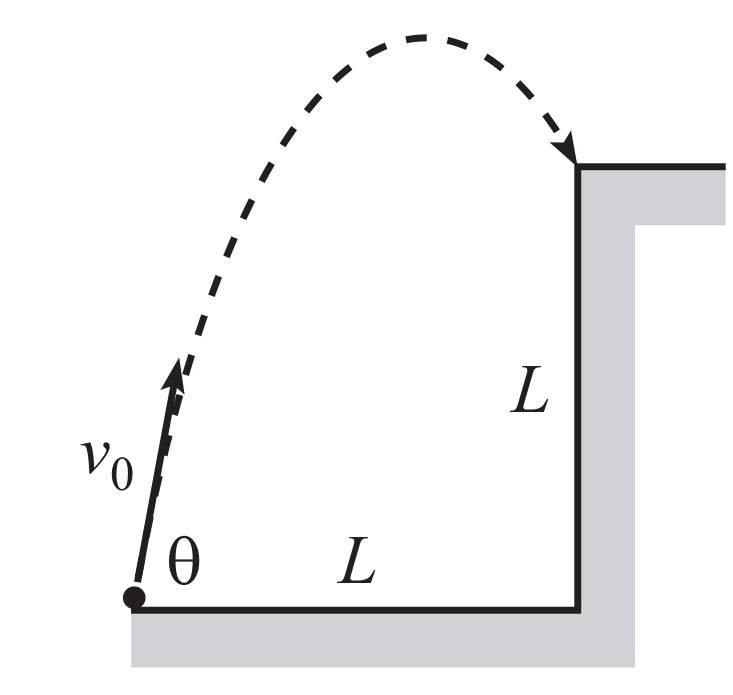
\includegraphics[width=0.45\linewidth]{figures/qfig1.png}
\end{center}

\begin{enumerate}
\item $\sqrt{\dfrac{gL}{2(\tan \theta - 1)}}$,
\item $\dfrac{1}{\cos \theta}\sqrt{\dfrac{gL}{2(\tan \theta - 1)}}$,
\item $\dfrac{1}{\cos \theta}\sqrt{\dfrac{gL}{2(\tan \theta + 1)}}$,
\item $\sqrt{\dfrac{gL \tan \theta}{2(\tan \theta + 1)}}$.
\end{enumerate}